\documentclass[10pt]{article}
% Formato extenso: report
\usepackage{subcaption}
% Removed sloppypar environment
% Formato corto: article

% Esto es para que el LaTeX sepa que el texto está en español:
\usepackage[english]{babel}

\usepackage{amsmath, amsthm, amsfonts,amssymb}

% Bórrame si quieres:
\usepackage{multicol}

% Referencias
\usepackage{hyperref}

% Paquete para escribir código
\usepackage{listings}
\lstset{basicstyle=\footnotesize\ttfamily,breaklines=true}
\usepackage{alltt}

% Paquete para incluir imágenes
\usepackage{graphicx}

% Paquete para incluir varias imágenes en una
\usepackage{subfig}

% para poder fijar las imágenes ([H])
\usepackage{float}

% para agregar opciones al enumerate
\usepackage{enumerate}

% Teoremas
\newtheorem{thm}{Teorema}[section]
\newtheorem{cor}[thm]{Corolario}
\newtheorem{lem}[thm]{Lema}
\newtheorem{prop}[thm]{Proposición}
\theoremstyle{definition}
\newtheorem{defn}[thm]{Definición}
\theoremstyle{remark}
\newtheorem{rem}[thm]{Observación}
\theoremstyle{definition}
\newtheorem{prob}{Problema}
\numberwithin{equation}{prob}

% Calculus symbols
\newcommand{\pd}[2]{\frac{\partial #1}{ \partial #2}}   % First partial derivative command
\newcommand{\td}[2]{\frac{\mathrm{d} #1}{ \mathrm{d} #2}}
\newcommand{\pdd}[2]{\frac{\partial^2 #1}{ \partial #2 ^2}}   % Second partial derivative command
\newcommand{\pddc}[3]{\frac{\partial^2 #1}{ \partial #2 \partial #3}}   % Second partial derivative command

% Continuum mechanics & FEM symbols
\def\sca   #1{\mbox{\rm{#1}}{}}
\def\mat   #1{\mbox{\boldmath $\mathsf #1$}}
\def\vec   #1{\mbox{\boldmath $#1$}{}}
\def\ten   #1{\mbox{\boldmath $#1$}{}}
\def\ltr   #1{\mbox{\sf{#1}}}
\def\bltr  #1{\mbox{\sffamily{\bfseries{{#1}}}}}

% math operators and symbols
\DeclareMathOperator{\dive}{div}
\DeclareMathOperator{\trace}{trace}
\DeclareMathOperator{\tr}{tr}
\DeclareMathOperator{\symm}{symm}
\DeclareMathOperator{\sk}{skew}
\DeclareMathOperator{\grad}{grad}
\DeclareMathOperator{\Grad}{Grad}
\DeclareMathOperator{\curl}{curl}
\DeclareMathOperator{\Curl}{Curl}
\def\R{\mbox{\(\mathbb{R}\)}}
\def\dx{\mbox{\(\,\mathrm{d}x\)}}


\usepackage{geometry}
\geometry{left=2.5cm, right=2.5cm, top=2cm, bottom=3cm}

\usepackage{makeidx}
\makeindex

\begin{document}


\begin{titlepage}


	%%%%% NO MODIFICAR
	\begin{figure}
		\begin{minipage}{4cm}
			
\includegraphics[width=0.9\textwidth]{./figures/logo}
		\end{minipage}
		\begin{minipage}{11cm}
			\vspace{4mm}
			{\sc UNIVERSIDAD DE VALPARAÍSO}\\
			Escuela de Ingeniería Civil Biomédica\\
			{\bf CBM414 Procesamiento digital de señales biomédicas}\\
			\vspace{0mm}
			\hrulefill
		\end{minipage}
	\end{figure}
	\phantom{""}\vspace{60mm}


	%%%%% MODIFICAR
	\begin{center}
		\Huge{\textbf{Laboratory 4}}\vspace{95mm}\\
		\raggedleft \Large{Maximiliano Antonio Gaete Pizarro}\\
	\end{center}


\end{titlepage}

\printindex

\tableofcontents

\newpage

\section{Time-Domain Comparison of Windows}
The following figure shows the time-domain comparison of the Rectangular, Hamming, and Hann windows of length $N = 128$.

\textbf{Python Code:}
\begin{lstlisting}[language=Python]
	import numpy as np
	import matplotlib.pyplot as plt
	from scipy.signal import get_window
	from scipy.fft import fft, fftshift, fftfreq
		
	# Window size
	N = 128
		
	# Generate the windows
	rectangular_window = get_window('boxcar', N)
	hamming_window = get_window('hamming', N)
	hann_window = get_window('hann', N)
		
	# Create the time axis
	n = np.arange(N)
		
	# Plot the windows
	plt.figure(figsize=(10, 6))
	plt.plot(n, rectangular_window, label='Rectangular (boxcar)', linestyle='-', marker='o')
	plt.plot(n, hamming_window, label='Hamming', linestyle='-', marker='x')
	plt.plot(n, hann_window, label='Hann', linestyle='-', marker='d')
		
	# Configure labels and legends
	plt.title('Comparison of Windows: Rectangular, Hamming, and Hann')
	plt.xlabel('Samples')
	plt.ylabel('Amplitude')
	plt.legend()
	plt.grid(True)
	plt.show()
\end{lstlisting}

\begin{figure}[H]
	\centering
	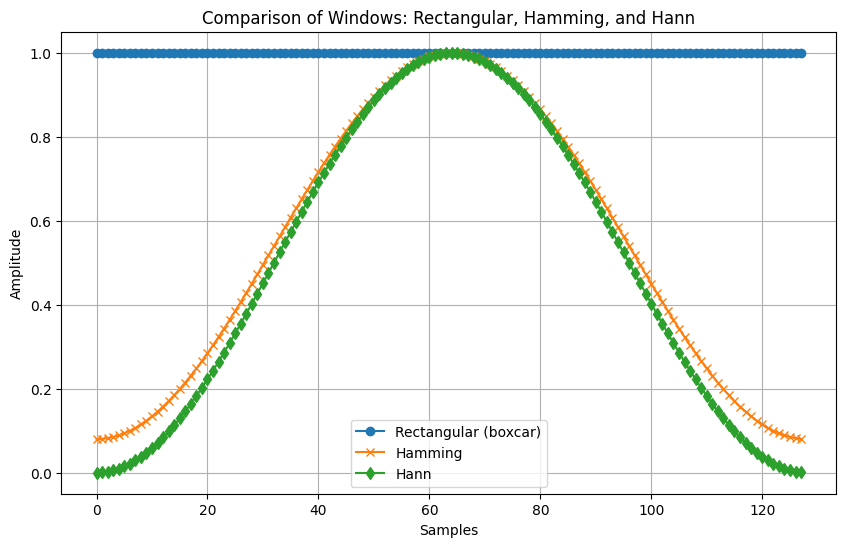
\includegraphics[width=0.7\textwidth]{./figures/Comparison of Windows.png}
	\caption{Comparison of Rectangular, Hamming, and Hann windows in the time domain.}
	\label{fig:time_domain}
\end{figure}

\newpage
	
\subsection*{Observations}
In the time domain, the three windows show distinct characteristics, summarized as follows:

\begin{itemize}
    \item \textbf{Rectangular Window:} The window maintains a constant amplitude of 1 across its entire length, which results in a sharp cut-off at the edges. This behavior leads to significant spectral leakage in the frequency domain.
    
    \item \textbf{Hamming Window:} The Hamming window tapers smoothly towards the edges, although it does not reach zero. This gradual tapering helps in reducing spectral leakage while maintaining relatively good frequency resolution.
    
    \item \textbf{Hann Window:} The Hann window also tapers smoothly, but unlike the Hamming window, it reaches an amplitude of zero at the edges. This smooth tapering to zero provides better suppression of leakage, though at the cost of wider main lobes in the frequency domain.
\end{itemize}


\subsection{Frequency-Domain Comparison of Windows}
The Fourier Transforms of the Rectangular, Hamming, and Hann windows are computed, and their magnitude spectra are shown below.

\textbf{Python Code:}
\begin{lstlisting}[language=Python]
# Zero padding for FFT
zero_pad = 10000

# Apply FFT with zero padding and avoid log10(0) by adding a small epsilon value
epsilon = 1e-10  # Small value to avoid log(0)
rectangular_fft = 10 * np.log10(2 / zero_pad * (np.abs(fftshift(fft(rectangular_window, zero_pad))) + epsilon))
hamming_fft = 10 * np.log10(2 / zero_pad * (np.abs(fftshift(fft(hamming_window, zero_pad))) + epsilon))
hann_fft = 10 * np.log10(2 / zero_pad * (np.abs(fftshift(fft(hann_window, zero_pad))) + epsilon))

# Generate the corresponding frequencies
freqs = fftshift(fftfreq(zero_pad))

# Plot the spectra
plt.figure(figsize=(10, 6))
plt.plot(freqs, rectangular_fft, label='Rectangular (boxcar)')
plt.plot(freqs, hamming_fft, label='Hamming')
plt.plot(freqs, hann_fft, label='Hann')

# Configure labels and legend
plt.title('Magnitude Spectrum of Windows: Rectangular, Hamming, and Hann')
plt.xlabel('Normalized Frequency')
plt.ylabel('Magnitude (dB)')
plt.legend()
plt.grid(True)
plt.xlim([-0.05, 0.05])  # Limit the X-axis to better view the main lobe
plt.show()
\end{lstlisting}
\begin{figure}[H]
	\centering
	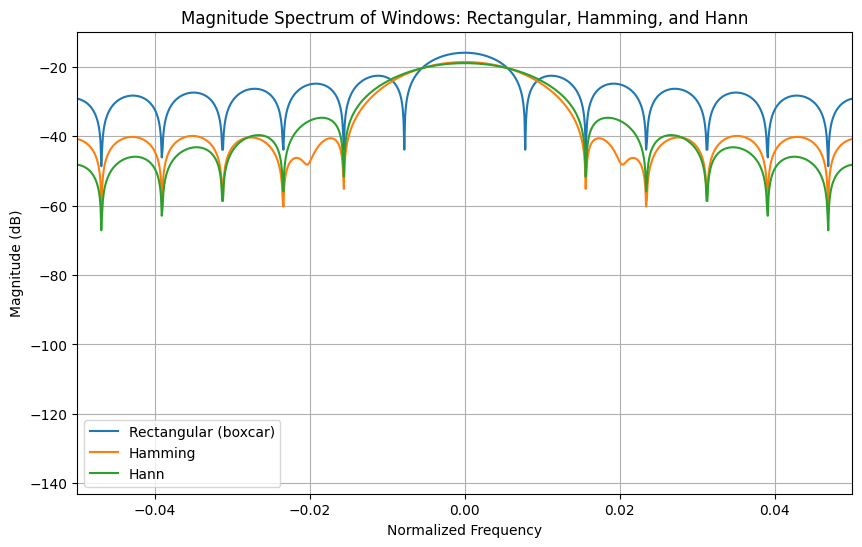
\includegraphics[width=0.6\textwidth]{./figures/Magnitude Spectrum of Windows.png}
	\caption{Magnitude spectrum of Rectangular, Hamming, and Hann windows.}
	\label{fig:freq_domain}
\end{figure}

\subsection*{Observations}
The analysis of the magnitude spectrum of the Rectangular, Hamming, and Hann windows leads to the following key observations:

\begin{itemize}
    \item \textbf{Rectangular Window:} This window exhibits the narrowest main lobe, which provides superior frequency resolution. However, it also presents the highest side lobes, causing significant spectral leakage. This makes it less suitable when side-lobe suppression is important.
    
    \item \textbf{Hamming Window:} The main lobe of the Hamming window is wider compared to the Rectangular window, which results in slightly lower frequency resolution. Nevertheless, the side lobes are considerably smaller, leading to reduced spectral leakage.
    
    \item \textbf{Hann Window:} Among the three, the Hann window has the widest main lobe, thus offering the lowest frequency resolution. However, its side lobes are the smallest, providing the best suppression of spectral leakage. This makes it particularly effective in applications where leakage minimization is prioritized.
\end{itemize}

\subsection{Discussion of Time-Domain and Frequency-Domain Representation}
The time-domain shape of a window has a direct influence on its behavior in the frequency domain:

\begin{itemize}
    \item A \textbf{sharp cutoff} in the time domain, as seen with the Rectangular window, results in a narrow main lobe but produces large side lobes in the frequency domain. This translates into higher spectral leakage.

    \item \textbf{Smoother transitions}, as observed with the Hamming and Hann windows, lead to significantly better suppression of the side lobes in the frequency domain. However, this improvement in leakage suppression comes at the cost of a wider main lobe, which reduces frequency resolution.
\end{itemize}

Thus, there is a clear trade-off between leakage suppression and frequency resolution. The Hann window provides the best side-lobe suppression, while the Rectangular window excels in frequency resolution. The Hamming window offers a balanced compromise between these two factors.

\subsection{Trade-offs in Window Selection}
When comparing the windows, the trade-off between frequency resolution and spectral leakage becomes evident:

\begin{itemize}
    \item The \textbf{Rectangular window} has the narrowest main lobe, giving it the best frequency resolution, but it also suffers from the worst spectral leakage due to high side lobes.
    
    \item The \textbf{Hamming window} offers a moderate compromise, with reduced spectral leakage at the expense of some frequency resolution. This balance makes it suitable for many practical signal processing tasks.
    
    \item The \textbf{Hann window}, with the widest main lobe, provides the best suppression of spectral leakage. However, the trade-off is that it offers the least frequency resolution. It is ideal for applications where leakage minimization is more important than precise frequency resolution.
\end{itemize}

In most practical applications, the \textbf{Hamming window} is often preferred as it strikes a good balance between frequency resolution and spectral leakage suppression, making it versatile for a variety of signal processing needs.





\section{Time-Domain Signal Visualization}

We start by visualizing both the resting and sleep signals in the time domain to observe their characteristics.

\begin{lstlisting}[language=Python]
	# Function to load a signal from a .txt file
	def load_signal_from_txt(filename, total_time=10):
		# Load the signal from the .txt file
		signal = np.loadtxt(filename, delimiter=';')[0, :]
		fs = np.round(len(signal)) / total_time
		# Return the loaded signal
		return signal, int(fs)

	reposo, fs_reposo = load_signal_from_txt('./reposo.txt')

	plt.figure(figsize=(10, 6))
	plt.plot(np.linspace(0, 10, 10 * fs_reposo), reposo, label=r'$\sigma = 1$')
	plt.title('Rest Signal in Time Domain')
	plt.xlabel('Time (s)')
	plt.ylabel('Amplitude')
	plt.legend()

	sueno, fs_sueno = load_signal_from_txt('./sueno.txt')

	plt.figure(figsize=(10, 6))
	plt.plot(np.linspace(0, 10, 10 * fs_sueno), sueno, label=r'$\sigma = 1$')
	plt.title('Sleep Signal in Time Domain')
	plt.xlabel('Time (s)')
	plt.ylabel('Amplitude')
	plt.legend()
	plt.show()
\end{lstlisting}


In the time domain, we can observe the amplitude and variability of the cardiac signals. Below are two figures representing the signals during rest and sleep.

\begin{figure}[H]
    \centering
    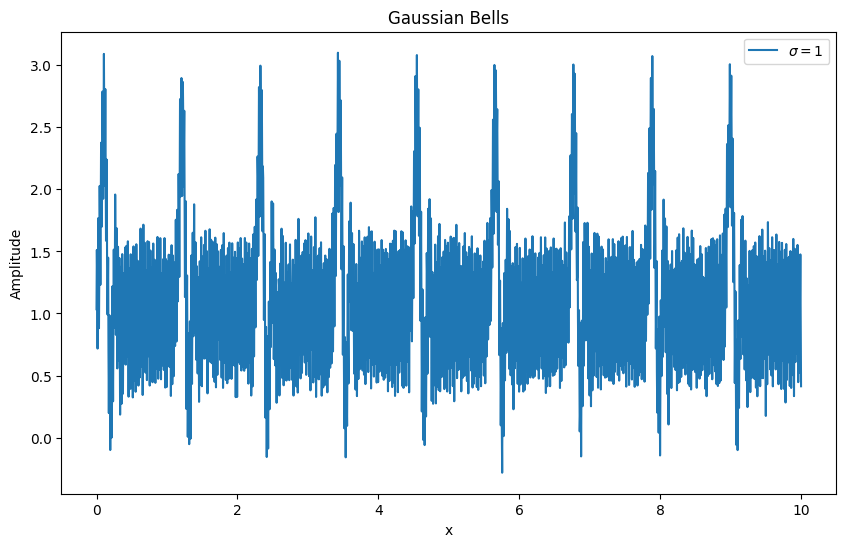
\includegraphics[width=0.8\textwidth]{./figures/Gaussian Bells Rest.png}
    \caption{Cardiac signal during rest (Time domain).}
    \label{fig:rest_signal}
\end{figure}

\begin{figure}[H]
    \centering
    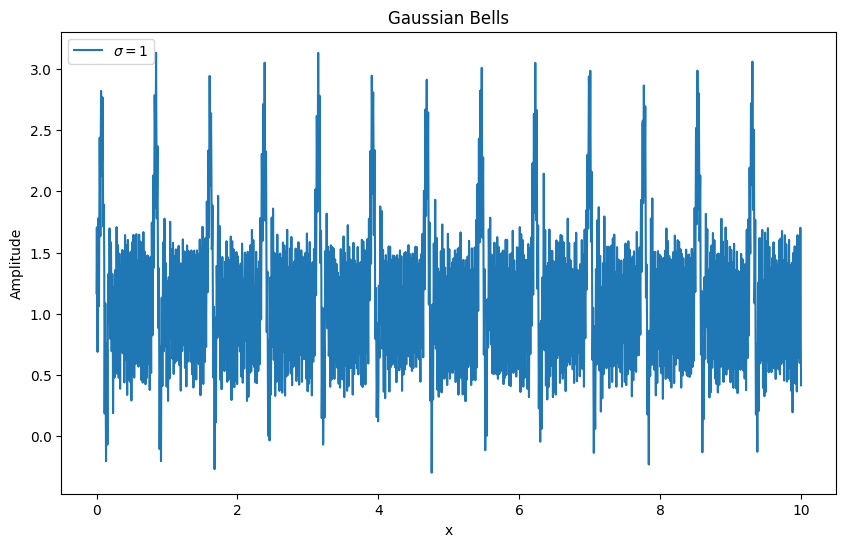
\includegraphics[width=0.8\textwidth]{./figures/Gaussian Bells Sleep.png}
    \caption{Cardiac signal during sleep (Time domain).}
    \label{fig:sleep_signal}
\end{figure}

From the figures, we can observe the following:

\begin{itemize}
    \item \textbf{Amplitude and variability:} The rest signal appears to have more regular amplitudes, while the sleep signal exhibits more irregularities in amplitude, which may correspond to different stages of sleep.
    \item \textbf{Peak frequency:} Peaks in the rest signal seem more evenly spaced compared to the sleep signal, indicating a more regular heartbeat during rest.
\end{itemize}

While time-domain analysis provides valuable information regarding amplitude and rhythm, it is insufficient for understanding the frequency characteristics of the cardiac signal. To overcome this limitation, frequency-domain analysis is necessary.

\subsection{Limitations of Time-Domain Analysis}

The time-domain analysis is limited in its ability to decompose the signal into its constituent frequencies. Cardiac signals are complex, comprising multiple frequency components. These components can change dynamically over time, especially during different sleep phases. The time-domain approach does not allow for the clear identification of these dominant frequencies.

For example, while the rest state may be dominated by lower frequencies corresponding to a steady heart rhythm, during sleep, certain stages (such as REM sleep) may introduce higher frequency components. These frequency variations are not easily visible in the time-domain representation.

\subsubsection{Frequency-Domain Analysis: The Spectrogram}

To fully understand the cardiac signal and its frequency components, we employ the spectrogram, which represents how the frequencies in the signal evolve over time.

\begin{figure}[H]
    \centering
    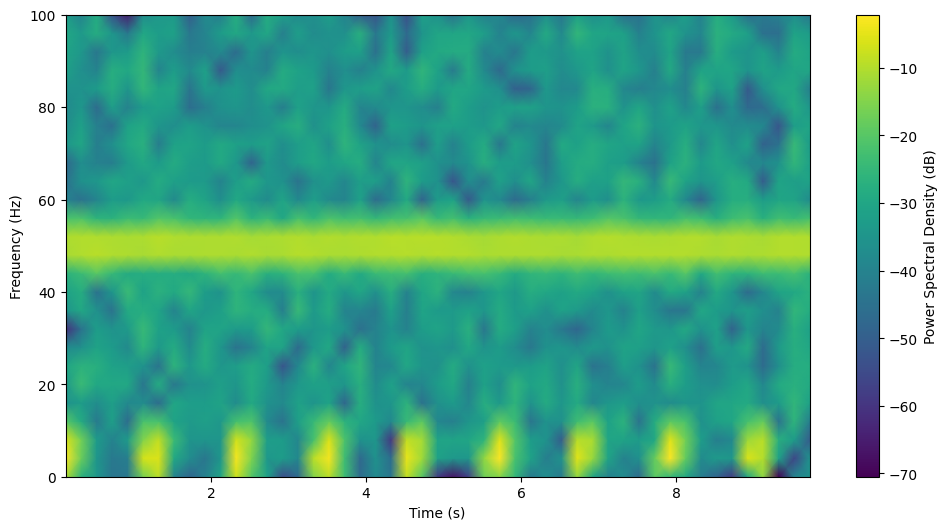
\includegraphics[width=0.8\textwidth]{./figures/Spectogram Rest.png}
    \caption{Spectrogram of the cardiac signal during rest.}
    \label{fig:spectrogram_rest}
\end{figure}

\begin{figure}[H]
    \centering
    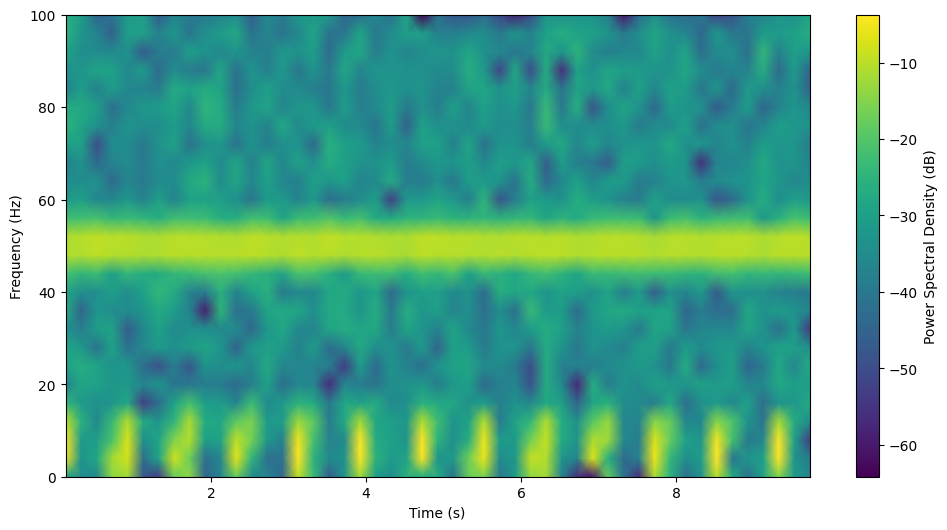
\includegraphics[width=0.8\textwidth]{./figures/Spectogram Sleep.png}
    \caption{Spectrogram of the cardiac signal during sleep.}
    \label{fig:spectrogram_sleep}
\end{figure}

The spectrogram provides the following advantages:

\begin{itemize}
    \item \textbf{Frequency evolution over time:} The spectrogram shows how the dominant frequencies change over time, a feature that is not accessible through time-domain analysis.
    \item \textbf{Power spectral density:} It displays the power of each frequency component, which is crucial for distinguishing relevant features of the signal from noise.
    \item \textbf{Identification of transitions:} The spectrogram allows for the identification of transitions between different phases, such as REM sleep, where the frequency content may change significantly.
\end{itemize}

\subsubsection{Low-Pass Filtering}

By observing the spectrogram, it becomes clear that a low-pass filter can be applied to isolate the lower frequencies associated with heartbeats. This filtering process can help in eliminating high-frequency noise or components that are not related to the heart's activity.

\begin{itemize}
    \item \textbf{Noise reduction:} By applying a low-pass filter, we can eliminate unwanted high-frequency noise, allowing for a clearer analysis of the heartbeats.
    \item \textbf{Heartbeat isolation:} The low-pass filter helps isolate the peaks and variability corresponding to heartbeats, making it easier to identify and analyze features such as heart rate variability (HRV).
    \item \textbf{Sleep phase analysis:} During different sleep phases, heart rhythms may change, but heartbeats remain the dominant feature in the lower frequency range. Applying a low-pass filter highlights these patterns more clearly and eliminates artifacts that could distort the signal interpretation.
\end{itemize}

\subsubsection{Conclusion}

In conclusion, while time-domain analysis gives a general overview of the signal's amplitude and rhythm, it is insufficient for understanding the signal's frequency characteristics. The spectrogram provides a more complete picture by revealing how the frequency content changes over time. Additionally, applying a low-pass filter further enhances the analysis by isolating the frequencies corresponding to heartbeats and reducing noise.









\subsection{Spectrograms with Different Window Types}

Now we compute and visualize the spectrograms using three window types: Rectangular, Hamming, and Hann. We use a window size of 256 samples and a 50\% overlap.

\begin{lstlisting}[language=Python]
from scipy import signal

# Define function to calculate and display the spectrogram
def plot_spectrogram(sig, fs, window_type='hann', window_size=256, overlapping=0.5, title=''):
    f, t, Sxx = signal.spectrogram(sig, fs, window=window_type, nperseg=window_size,
                                   noverlap=int(window_size * overlapping), scaling='spectrum')
    plt.figure(figsize=(12, 6))
    plt.pcolormesh(t, f, 10 * np.log10(Sxx), shading='gouraud')
    plt.colorbar(label='Power Spectral Density (dB)')
    plt.ylabel('Frequency (Hz)')
    plt.xlabel('Time (s)')
    plt.title(title)
    plt.show()

# Common parameters
window_size = 256
overlapping = 0.5

# List of windows
windows = ['boxcar', 'hamming', 'hann']
window_names = ['Rectangular', 'Hamming', 'Hann']

# Signal at rest
for window, name in zip(windows, window_names):
    plot_spectrogram(reposo, fs_reposo, window_type=window, window_size=window_size,
                     overlapping=overlapping, title=f'Spectrogram (Rest) - Window {name}')

# Signal during sleep
for window, name in zip(windows, window_names):
    plot_spectrogram(sueno, fs_sueno, window_type=window, window_size=window_size,
                     overlapping=overlapping, title=f'Spectrogram (Sleep) - Window {name}')
\end{lstlisting}


\subsection*{Rest Signal Spectrograms}

\subsubsection{Rectangular Window}
The rectangular window is the simplest, with no weighting applied. As a result, it suffers from aliasing and spectral leakage, meaning it is less effective at separating closely spaced frequency components. In the spectrogram, this is reflected in less defined frequency lines and more ``noise'' surrounding the actual frequencies.

\begin{figure}[H]
    \centering
    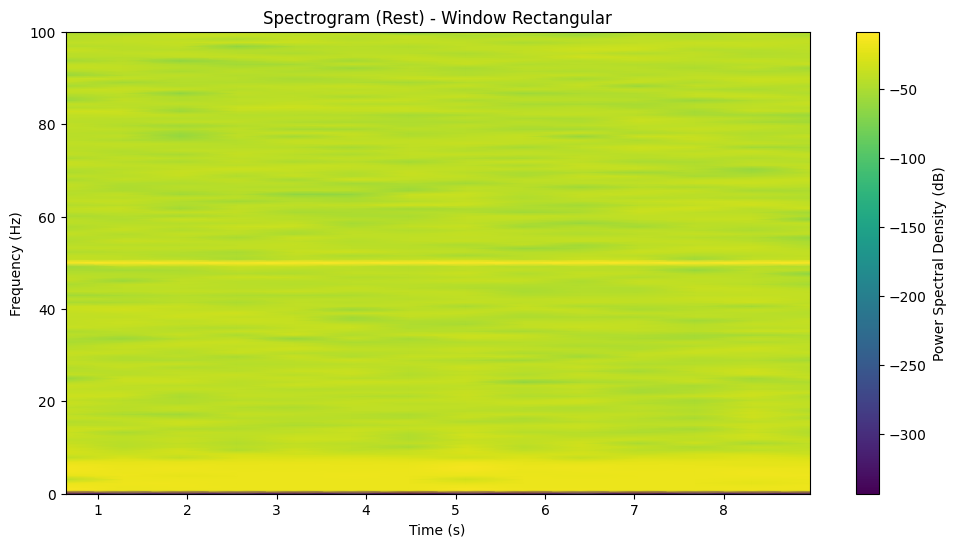
\includegraphics[width=0.7\textwidth]{./figures/Spectrogram (Rest) - Window Rectangular.png}
    \caption{Spectrogram (Rest) using Rectangular Window}
\end{figure}

\subsubsection{Hamming Window}
The Hamming window smooths the edges, reducing spectral leakage. This means that the frequency components in the spectrogram are more defined compared to the rectangular window but at the cost of lower time resolution. The energy of the frequency components is more concentrated, making individual frequencies easier to identify.

\begin{figure}[H]
    \centering
    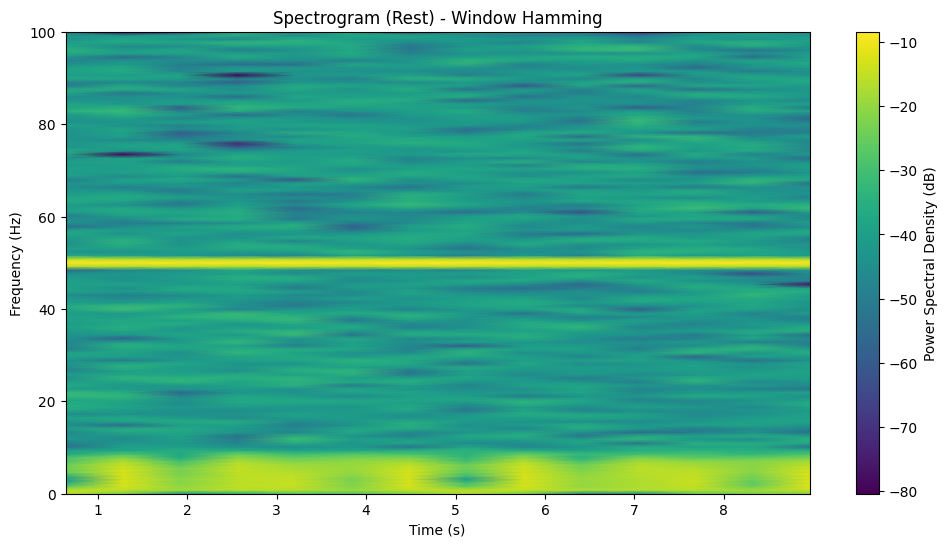
\includegraphics[width=0.7\textwidth]{./figures/Spectrogram (Rest) - Window Hamming.png}
    \caption{Spectrogram (Rest) using Hamming Window}
\end{figure}

\subsubsection{Hann Window}
The Hann window is similar to the Hamming window but with a steeper fall-off at the edges, making it ideal for periodic signals. The spectrogram shows an energy distribution that is intermediate between the rectangular and Hamming windows, with well-defined frequency components but slightly worse time resolution than the rectangular window.

\begin{figure}[H]
    \centering
    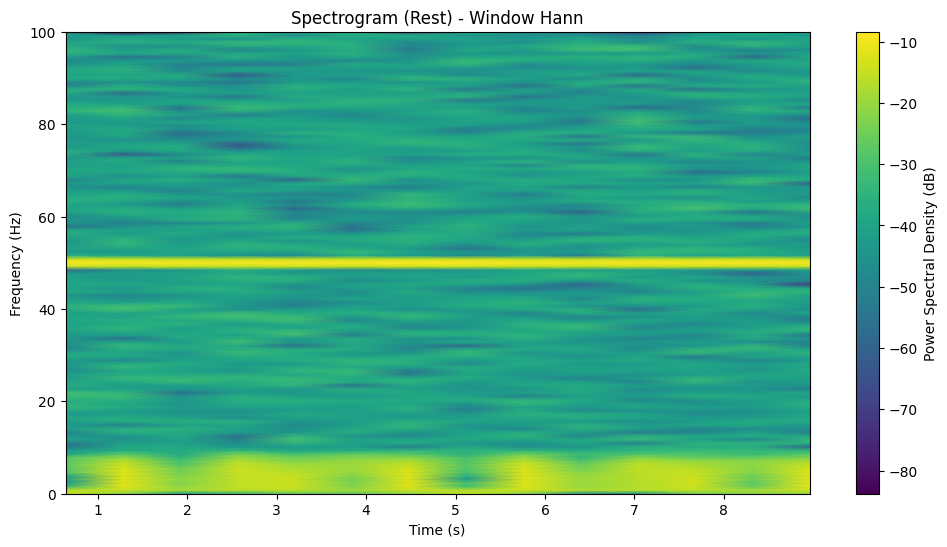
\includegraphics[width=0.7\textwidth]{./figures/Spectrogram (Rest) - Window Hann.png}
    \caption{Spectrogram (Rest) using Hann Window}
\end{figure}


\subsection{Sleep Signal Spectrograms}

\subsubsection{Rectangular Window}
Due to high spectral leakage, the rectangular window tends to show additional frequency components that are not actually present in the signal. This occurs because the transitions between different frequency components are not smoothed, leading to artifacts.

\begin{figure}[H]
    \centering
    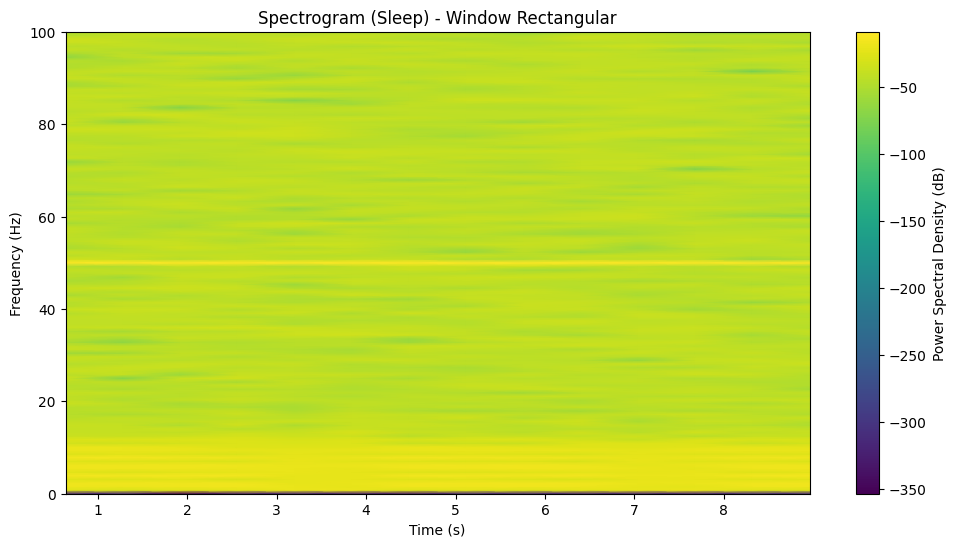
\includegraphics[width=0.7\textwidth]{./figures/Spectrogram (Sleep) - Window Rectangular.png}
    \caption{Spectrogram (Sleep) using Rectangular Window}
\end{figure}

\subsubsection{Hamming Window}
This window minimizes the appearance of spurious components, making the spectrogram more faithful to the actual frequency components of the signal. The primary frequencies will be better differentiated and less affected by artifacts.

\begin{figure}[H]
    \centering
    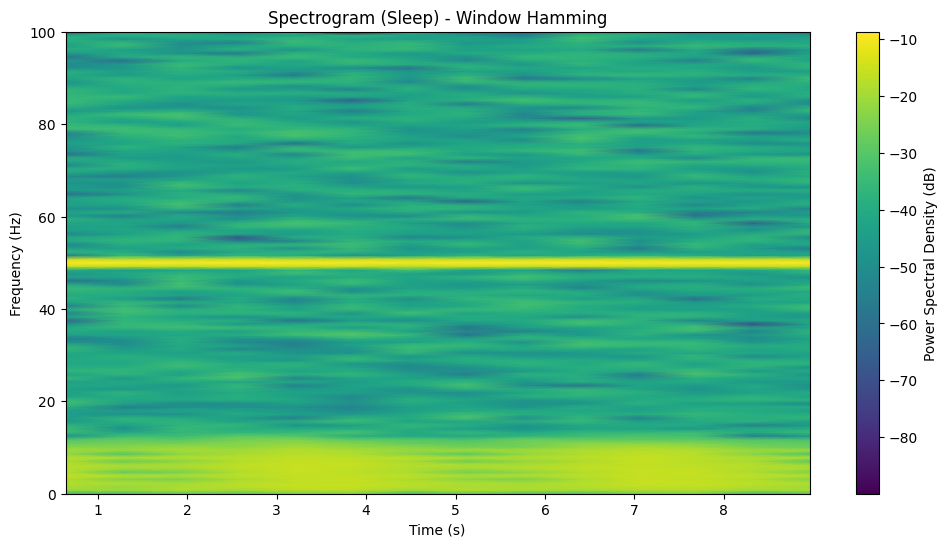
\includegraphics[width=0.7\textwidth]{./figures/Spectrogram (Sleep) - Window Hamming.png}
    \caption{Spectrogram (Sleep) using Hamming Window}
\end{figure}

\subsubsection{Hann Window}
Like the Hamming window, the Hann window suppresses spurious components, but its faster fall-off at the edges means that frequencies very close together may appear more overlapped compared to the Hamming window.

\begin{figure}[H]
    \centering
    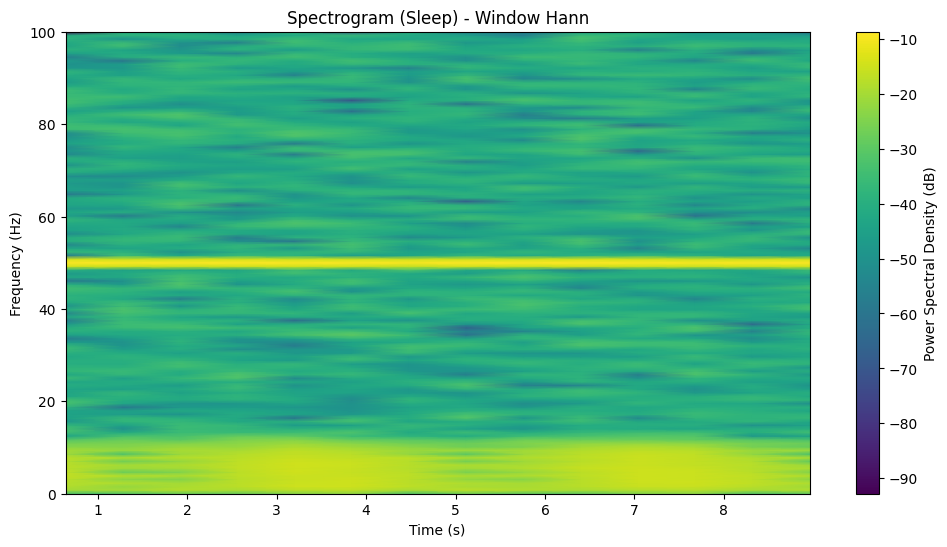
\includegraphics[width=0.7\textwidth]{./figures/Spectrogram (Sleep) - Window Hann.png}
    \caption{Spectrogram (Sleep) using Hann Window}
\end{figure}


\subsection{Energy Distribution}

\subsubsection{Rectangular Window}
The energy distribution is more dispersed with the rectangular window. Spectral leakage is more noticeable, leading to a less accurate representation of the frequency components. This can make adjacent frequencies appear more diffuse.

\subsubsection{Hamming Window}
With this window, the energy is more concentrated around the main frequencies. In the spectrogram, this results in more defined frequency components and less noise between them.

\subsubsection{Hann Window}
The Hann window provides a concentration of energy that is slightly less than the Hamming window but better than the rectangular window. The frequency components in the spectrogram are clear, though the additional smoothness of the window may cause some detail to be lost in rapid frequency transitions.


\section*{Conclusion}

Each window affects both the time and frequency resolution of the spectrograms. The Rectangular window offers the best time resolution but poor frequency resolution, introducing more artifacts. On the other hand, the Hamming and Hann windows provide better frequency resolution, which allows for clearer spectral components at the expense of time resolution. For signals with well-defined frequency components where spectral noise is a concern, Hamming or Hann windows are preferable, while the rectangular window may be chosen when time resolution is more critical.



\section{ffect of Different Overlaps with Hamming Window}

Next, we analyze the effect of different overlap percentages: 0\%, 50\%, and 75\%, while using the Hamming window and a window size of 256 samples.



\begin{lstlisting}[language=Python]
# List of overlap percentages
overlaps = [0.0, 0.5, 0.75]
overlap_percentages = ['0%', '50%', '75%']

# Signal at rest with different overlaps
for overlap, percentage in zip(overlaps, overlap_percentages):
    plot_spectrogram(reposo, fs_reposo, window_type='hamming', window_size=256,
                     overlapping=overlap, title=f'Spectrogram (Rest) - Overlap {percentage}')

# Signal during sleep with different overlaps
for overlap, percentage in zip(overlaps, overlap_percentages):
    plot_spectrogram(sueno, fs_sueno, window_type='hamming', window_size=256,
                     overlapping=overlap, title=f'Spectrogram (Sleep) - Overlap {percentage}')
\end{lstlisting}

\subsection{Rest Spectrogram Analysis}

\subsubsection{Overlap 0\%}
In the spectrogram with no overlap (0\%), we observe that the data representation is rougher and less smooth. Transitions between different frequency bands and power levels appear less continuous, which results in a higher capacity to capture sudden changes in the signal over time. However, this increased temporal resolution comes at the cost of lower frequency resolution, meaning finer details in the frequency domain might not be as prominent.

\begin{figure}[H]
    \centering
    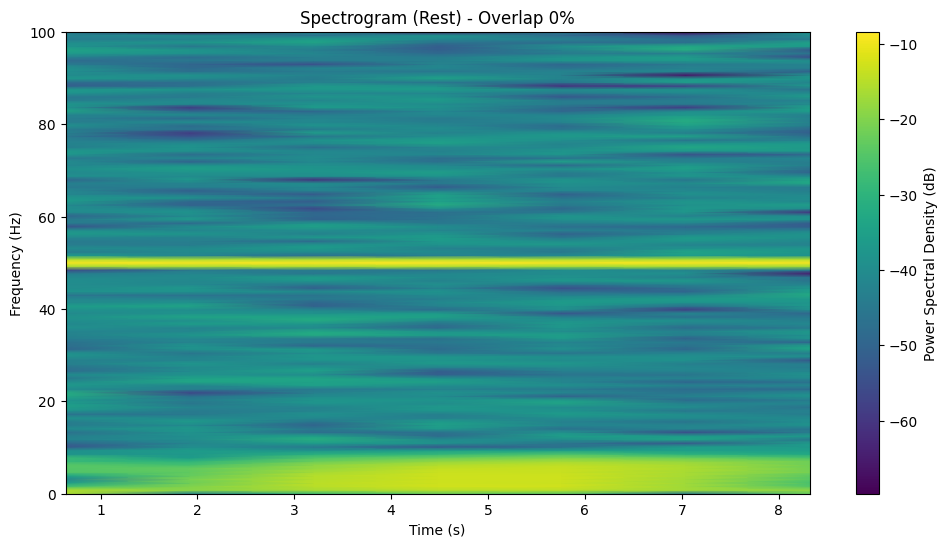
\includegraphics[width=0.8\textwidth]{./figures/Spectrogram (Rest) - Overlap 0.png}
    \caption{Spectrogram (Rest) with 0\% Overlap}
    \label{fig:rest_0_overlap}
\end{figure}


\subsubsection{Overlap 50\%}
As the overlap increases to 50\%, we observe a balance between temporal resolution and smoothness. Changes in the signal are captured more precisely in both domains without sacrificing too much temporal or frequency resolution. This overlap is typically seen as a good compromise, as it improves the continuity of transitions in the spectrogram without losing too much temporal information.

\begin{figure}[H]
    \centering
    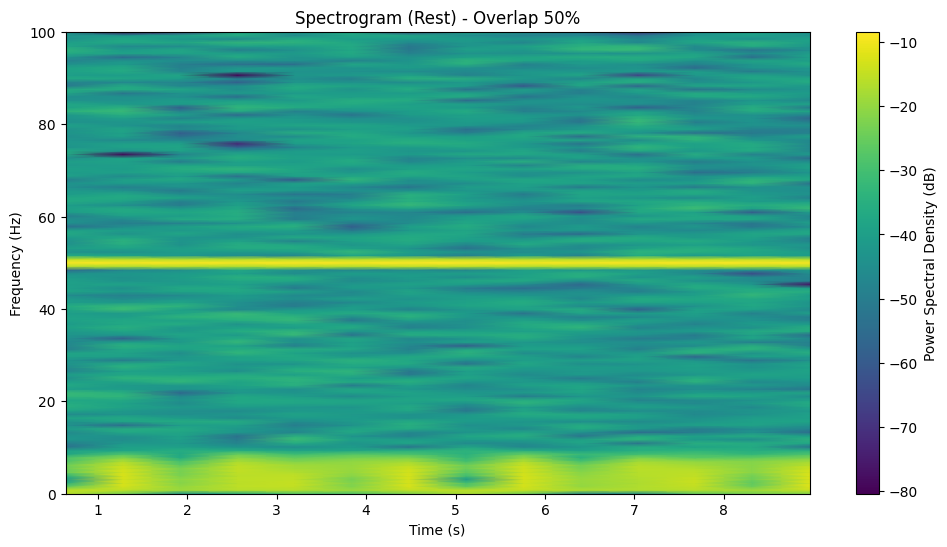
\includegraphics[width=0.8\textwidth]{./figures/Spectrogram (Rest) - Overlap 50.png}
    \caption{Spectrogram (Rest) with 50\% Overlap}
    \label{fig:rest_50_overlap}
\end{figure}

\subsubsection{Overlap 75\%}
With a 75\% overlap, the spectrogram appears much smoother. This results in a more continuous representation of frequency bands, making it easier to visualize more persistent or longer-duration frequency components. However, this smoothness reduces the ability to detect rapid changes in time, as temporal resolution is compromised. Nevertheless, frequency resolution is improved, focusing on stationary characteristics of the signal.

\begin{figure}[H]
    \centering
    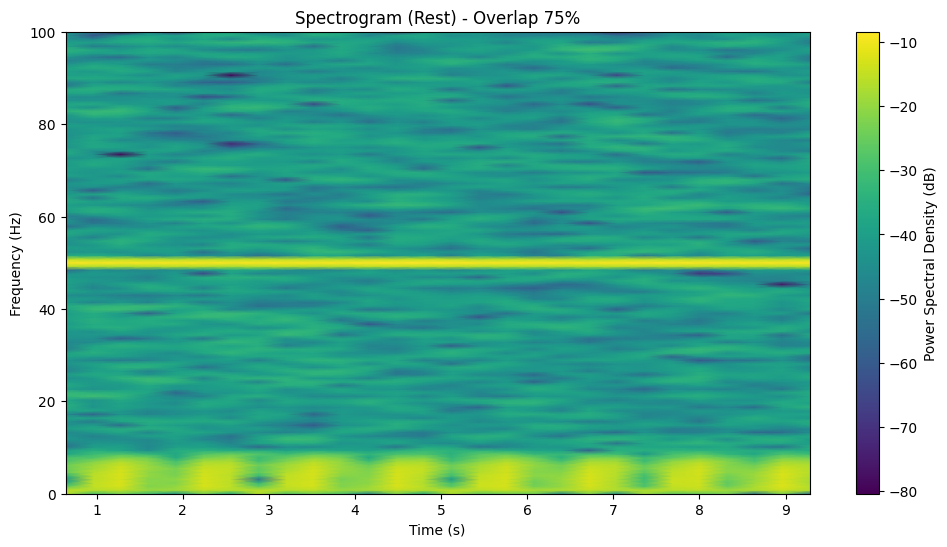
\includegraphics[width=0.8\textwidth]{./figures/Spectrogram (Rest) - Overlap 75.png}
    \caption{Spectrogram (Rest) with 75\% Overlap}
    \label{fig:rest_75_overlap}
\end{figure}


\subsection{Sleep Spectrogram Analysis}

To further understand this effect, we see the spectrogram for a sleep condition with varying overlaps.

\subsubsection{Overlap 0\%}
\begin{figure}[H]
    \centering
    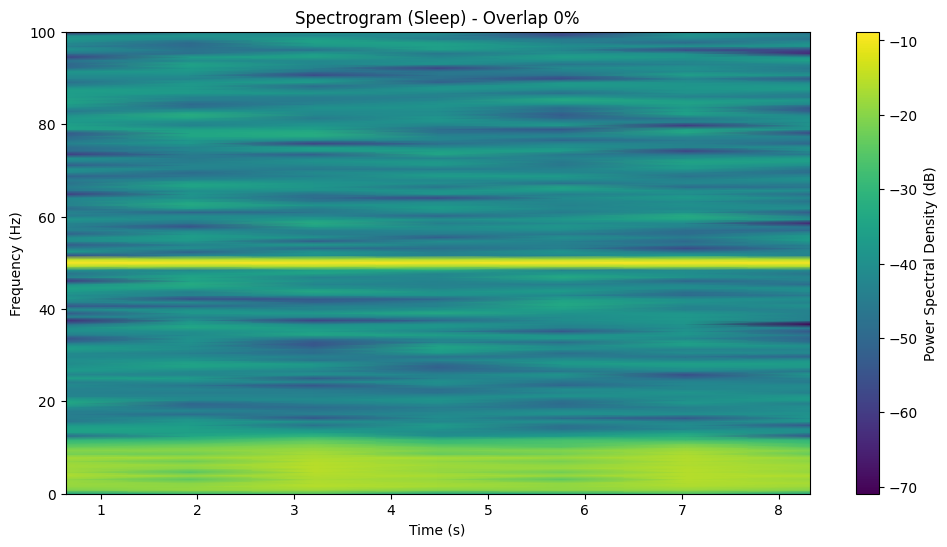
\includegraphics[width=0.8\textwidth]{./figures/Spectrogram (Sleep) - Overlap 0.png}
    \caption{Spectrogram (Sleep) with 0\% Overlap}
    \label{fig:sleep_0_overlap}
\end{figure}

\subsubsection{Overlap 50\%}
\begin{figure}[H]
    \centering
    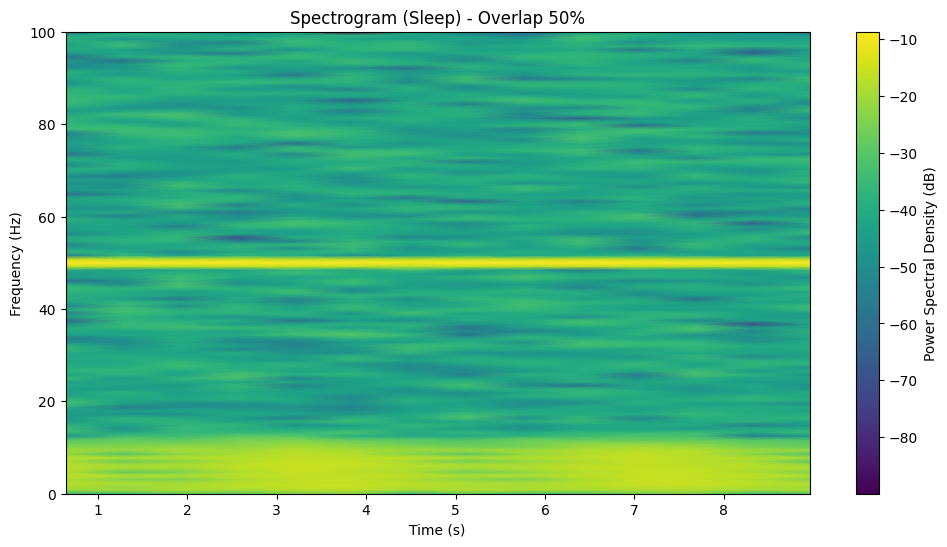
\includegraphics[width=0.8\textwidth]{./figures/Spectrogram (Sleep) - Overlap 50.png}
    \caption{Spectrogram (Sleep) with 50\% Overlap}
    \label{fig:sleep_50_overlap}
\end{figure}

\subsubsection{Overlap 75\%}

\begin{figure}[H]
    \centering
    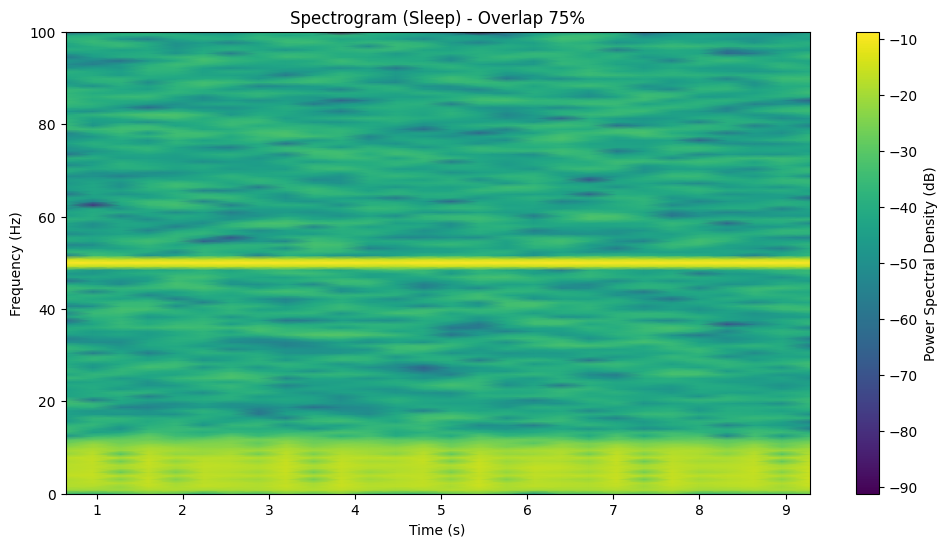
\includegraphics[width=0.8\textwidth]{./figures/Spectrogram (Sleep) - Overlap 75.png}
    \caption{Spectrogram (Sleep) with 75\% Overlap}
    \label{fig:sleep_75_overlap}
\end{figure}

\subsection{Relation to the Heisenberg Uncertainty Principle}

The Heisenberg Uncertainty Principle, when applied to signal analysis, states that there is a trade-off between time and frequency resolution. It is not possible to improve both simultaneously; increasing the resolution in time results in a loss of frequency precision, and vice versa.

\subsection*{Temporal Resolution}
Temporal resolution refers to the ability to identify changes in the signal over short time intervals. A lower overlap (0\%) enhances temporal resolution, allowing transient events to be captured more clearly, but sacrifices the ability to represent frequencies accurately.

\subsection*{Frequency Resolution}
Frequency resolution represents the ability to distinguish between nearby frequencies. A higher overlap (50\% or 75\%) improves frequency resolution, allowing more persistent or subtle frequency components to be identified. However, this comes at the cost of detecting rapid changes in time.

The window size (256 samples in this case) plays a crucial role in this trade-off. Larger windows offer better frequency resolution at the cost of temporal resolution, and vice versa. By applying overlap, especially in combination with smaller windows, it is possible to improve frequency resolution without losing too much temporal information.

\section*{Conclusion}

In summary, overlap affects the smoothness of the spectrogram and the ability to detect rapid changes in the signal as follows:
\begin{itemize}
    \item Lower overlap (0\%) prioritizes temporal resolution at the expense of a noisier or less continuous frequency representation.
    \item Intermediate overlap (50\%) achieves a good compromise between temporal and frequency resolution.
    \item Higher overlap (75\%) improves smoothness and frequency precision but reduces the ability to capture transient events.
\end{itemize}

This analysis directly reflects the Heisenberg Uncertainty Principle, where increasing the resolution in one domain leads to a decrease in resolution in the other. The choice of overlap percentage and window size must be carefully selected based on the goal of the analysis, whether to detect transient events or highlight persistent frequency characteristics.






\section{Effect of Window Size on Spectrogram Resolution}

We now compare the spectrograms using different window sizes: 128, 256, and 512 samples, with a 50\% overlap.

\begin{lstlisting}[language=Python]
# List of window sizes
window_sizes = [128, 256, 512]
window_size_labels = ['128 samples', '256 samples', '512 samples']

# Spectrograms with different window sizes
for size, label in zip(window_sizes, window_size_labels):
    plot_spectrogram(reposo, fs_reposo, window_type='hamming', window_size=size,
                     overlapping=0.5, title=f'Spectrogram (Rest) - Window Size {label}')
\end{lstlisting}

\begin{figure}[H]
    \centering
    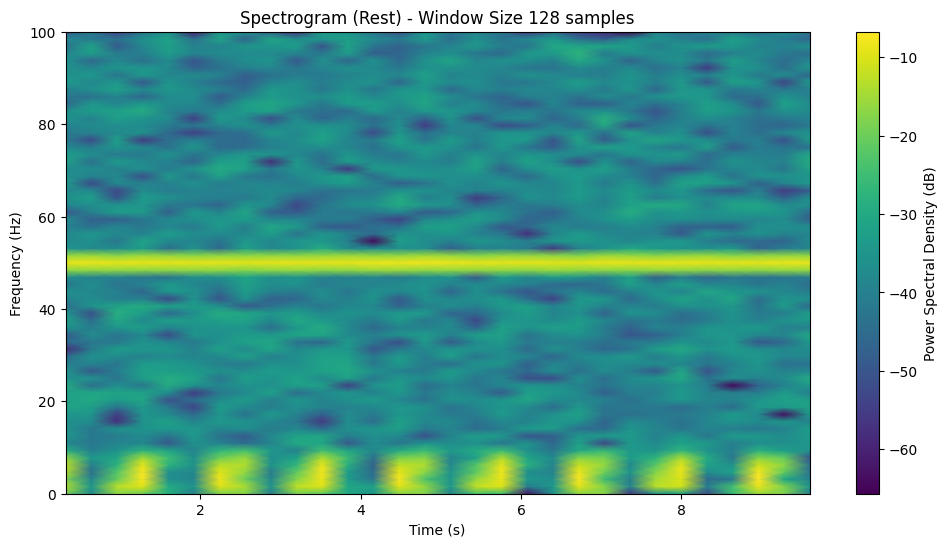
\includegraphics[width=0.7\textwidth]{./figures/Spectrogram (Rest) - Window Size 128 samples.png}
    \caption{Spectrogram with Window Size 128 samples}
    
    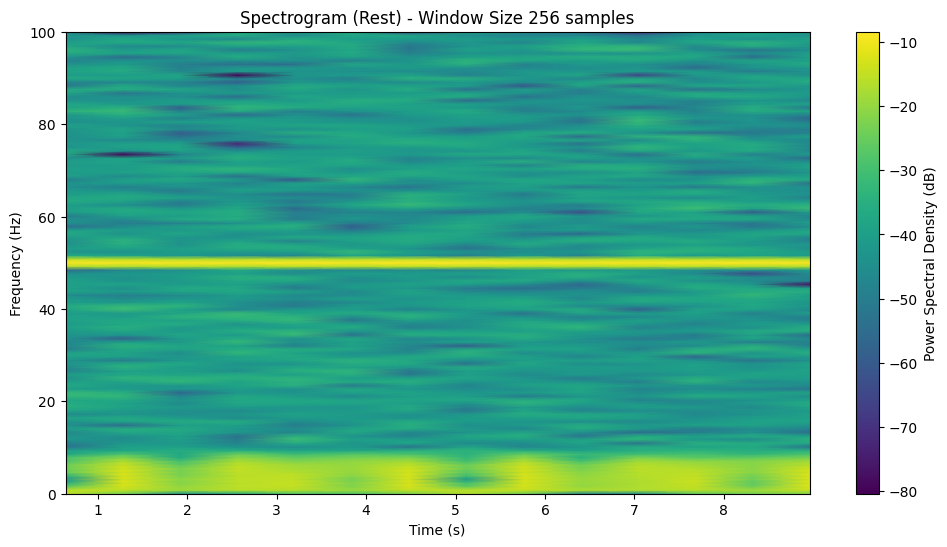
\includegraphics[width=0.7\textwidth]{./figures/Spectrogram (Rest) - Window Size 256 samples.png}
    \caption{Spectrogram with Window Size 256 samples}
    
    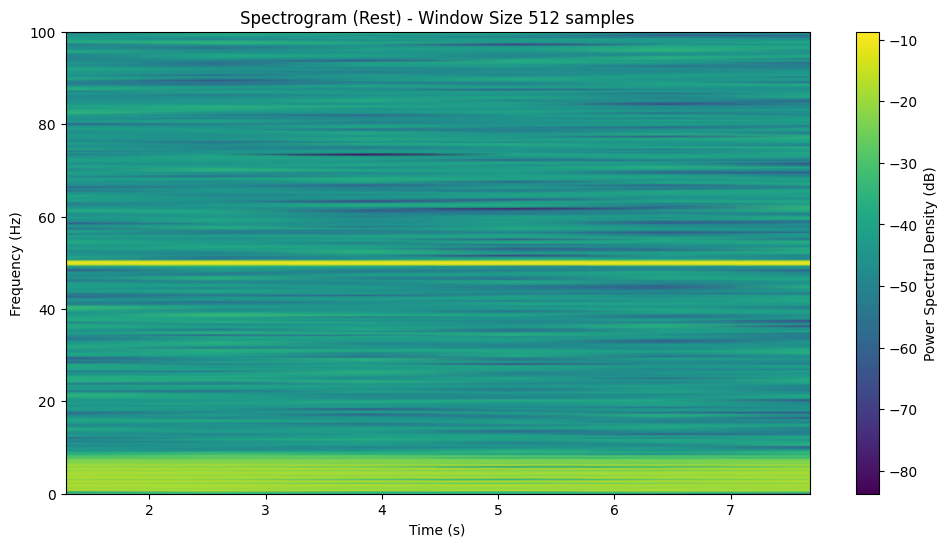
\includegraphics[width=0.7\textwidth]{./figures/Spectrogram (Rest) - Window Size 512 samples.png}
    \caption{Spectrogram with Window Size 512 samples}
    
    \label{fig:spectrograms}
\end{figure}

\subsection{Temporal Resolution}
Temporal resolution refers to the ability of the spectrogram to distinguish events over time. A smaller window size leads to better temporal resolution, meaning that it is easier to detect rapid changes in the signal.

\begin{itemize}
    \item With a window size of \textbf{128 samples}, we observe the highest temporal resolution. The variability along the time axis is more defined, and rapid changes in the signal are better captured, especially in the lower frequency ranges.
    \item Increasing the window size to \textbf{256 samples} reduces temporal resolution. Rapid transitions or changes in the signal become more diffuse, smoothing out variations.
    \item At a window size of \textbf{512 samples}, the temporal resolution is the lowest. The signal's rapid changes are significantly smoothed out and are less distinguishable.
\end{itemize}

\subsection{Frequency Resolution}
Frequency resolution refers to the ability of the spectrogram to distinguish between closely spaced frequencies. A larger window size leads to better frequency resolution.

\begin{itemize}
    \item With a window size of \textbf{128 samples}, the frequency resolution is limited. The frequency bands appear wider, making it harder to distinguish between adjacent frequencies.
    \item As the window size increases to \textbf{256 samples}, the frequency resolution improves, and closely spaced frequencies become more distinguishable.
    \item With a window size of \textbf{512 samples}, the frequency resolution is the highest, as the frequency bands are more sharply defined, particularly around 60 Hz.
\end{itemize}




\subsection{Ability to Detect Rapid Changes in Time}
\begin{itemize}
    \item The spectrogram with a \textbf{128-sample window} size offers the best ability to detect rapid changes in time, as the small window captures the quick transitions in the signal with high detail.
    \item As the window size increases to \textbf{256 and 512 samples}, the ability to detect rapid changes decreases. The signal becomes smoother over time, and fast transitions are averaged out, making them less noticeable.
\end{itemize}

\subsection*{Conclusion}
\begin{itemize}
    \item A smaller window size (128 samples) provides better \textbf{temporal resolution}, allowing the detection of rapid events in the signal at the cost of \textbf{frequency resolution}.
    \item A larger window size (512 samples) improves \textbf{frequency resolution}, enabling better distinction between closely spaced frequencies but at the expense of losing details of rapid changes over time.
    \item The intermediate window size (256 samples) balances both temporal and frequency resolution, but still sacrifices the ability to capture rapid temporal events.
\end{itemize}


\section{Best Combination of Parameters}

The analysis of cardiac signals using spectrograms requires a careful selection of parameters, such as the window type, window size, and overlap. These parameters directly influence the trade-off between temporal and frequency resolution, and thus the type of information that can be extracted from the spectrogram.

\subsection{Selection of Parameters}

For this analysis, the following parameters were chosen based on the optimal balance between temporal and frequency resolution:

\begin{itemize}
    \item \textbf{Window type}: Hamming
    \item \textbf{Window size}: 256 samples
    \item \textbf{Overlap}: 75\%
\end{itemize}

The Hamming window was selected due to its ability to provide a good compromise between minimizing spectral leakage and maintaining accurate frequency representation. A window size of 256 samples was chosen as it offers a good balance between capturing the variations in heart rate (temporal resolution) and resolving the frequency components of interest (frequency resolution). The 75\% overlap ensures that no information is lost between successive windows and that temporal continuity is preserved.

\subsection{Balancing Temporal and Frequency Resolution}

The choice of these parameters directly affects the resolution of the spectrogram:
\begin{itemize}
    \item \textbf{Temporal resolution}: A smaller window size improves temporal resolution, allowing the detection of rapid changes in the signal, such as individual heartbeats.
    \item \textbf{Frequency resolution}: A larger window size improves frequency resolution, allowing better identification of specific frequency components, such as heart rate variability.
\end{itemize}

With the selected window size of 256 samples, an appropriate balance is achieved, ensuring that both rapid changes and frequency components are accurately captured.

\subsection{Differences between Rest and Sleep States}

The cardiac signals during rest and sleep typically exhibit different characteristics. During rest, the signal is more stable, with less variability in heart rate. In contrast, during sleep, especially in REM sleep, the cardiovascular system shows higher variability, with fluctuations in heart rate being more pronounced.

\subsubsection{Resting Signal}

During rest, the spectrogram tends to show a clear dominant frequency corresponding to the average heart rate, with less variability over time. The selected parameters provide sufficient resolution to capture this steady behavior.

\subsubsection{Sleep Signal}

During sleep, the signal exhibits greater variability, particularly in the REM phase. The spectrogram shows transient increases in higher frequencies, reflecting increased sympathetic activity. The selected window size and overlap allow for the capture of these rapid changes, especially during the transition between sleep stages.

\subsection{Interpretation of Spectrograms}

The spectrograms obtained with the selected parameters reveal the following patterns:
\begin{itemize}
    \item \textbf{Rest}: A stable frequency component corresponding to the average heart rate, with low variability.
    \item \textbf{Sleep}: Higher variability, particularly during REM sleep, with transient increases in higher frequency components.
\end{itemize}

These changes in frequency components during sleep are related to the regulation of the autonomic nervous system, with increased sympathetic activity during REM sleep leading to higher heart rate variability.

\section*{Conclusion}

The chosen combination of window type (Hamming), window size (256 samples), and overlap (75\%) provides an optimal balance for analyzing cardiac signals in both rest and sleep states. The parameters allow for accurate capture of both the temporal dynamics of heart rate and its frequency components, enabling a comprehensive understanding of the cardiovascular system's behavior in different physiological states.

\begin{figure}[h]
    \centering
    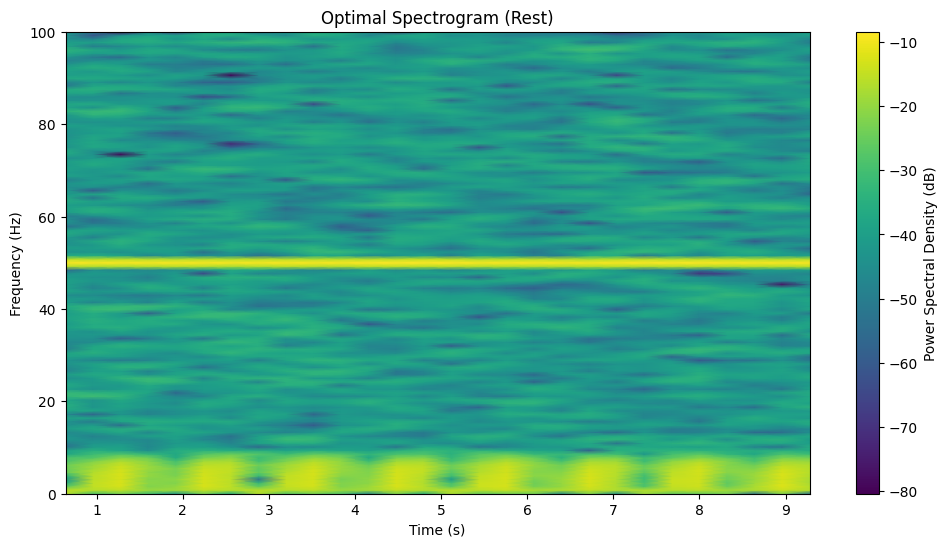
\includegraphics[width=0.7\textwidth]{./figures/Optimal Spectrogram (Rest).png}
    \caption{Spectrogram of the cardiac signal during rest.}
\end{figure}

\begin{figure}[h]
    \centering
    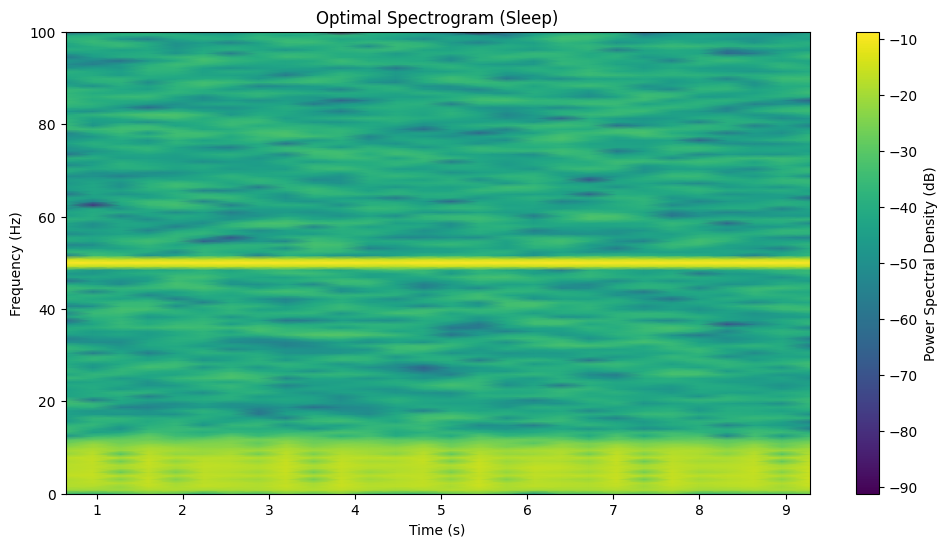
\includegraphics[width=0.7\textwidth]{./figures/Optimal Spectrogram (Sleep).png}
    \caption{Spectrogram of the cardiac signal during sleep.}
\end{figure}

\end{document}


